\section{Additional Tables and Figures}\label{app:tab_figures}

\begingroup
\footnotesize  % or \small, \scriptsize for even smaller
\setlength{\tabcolsep}{3pt}  % reduce column spacing
\renewcommand{\arraystretch}{1.0}  % reduce row height

\begin{longtable}{>{\raggedright\arraybackslash}p{0.3\textwidth}
                  >{\raggedright\arraybackslash}p{0.3\textwidth}
                  >{\raggedright\arraybackslash}p{0.3\textwidth}}
\caption{News Topics from \citet{Bybee2021}}
\label{tab:news_topics} \\
\toprule
\textbf{Topic} & \textbf{Topic} & \textbf{Topic} \\
\midrule
\endfirsthead

\multicolumn{3}{c}{\tablename\ \thetable\ -- \textit{Continued from previous page}} \\
\toprule
\textbf{Topic} & \textbf{Topic} & \textbf{Topic} \\
\midrule
\endhead

\midrule
\multicolumn{3}{r}{\textit{Continued on next page}} \\
\endfoot

\bottomrule
\endlastfoot

Natural disasters & Internet & Soft drinks \\
Mobile devices & Profits & M\&A \\
Changes & Police / crime & Research \\
Executive pay & Mid-size cities & Scenario analysis \\
Economic ideology & Middle East & Savings \& loans \\
IPOs & Restraint & Electronics \\
Record high & Connecticut & Steel \\
Bond yields & Small business & Cable \\
Fast food & Disease & Activists \\
Competition & Music industry & Short sales \\
Nonperforming loans & Key role & News conference \\
U.S. defense & Political contributions & Revised estimate \\
Economic growth & Justice Department & Credit ratings \\
Broadcasting & Problems & Announce plan \\
Federal Reserve & Job cuts & Chemicals / paper \\
Regulation & Environment & Small caps \\
Unions & C-suite & Control stakes \\
Mutual funds & Venture capital & European sovereign debt \\
Mining & Company spokesperson & Private / public sector \\
Pharma & Schools & Russia \\
Programs / initiatives & Health insurance & Drexel \\
Trade agreements & Treasury bonds & Challenges \\
People familiar & Sales call & Publishing \\
Financial crisis & Aerospace / defense & Recession \\
Latin America & Cultural life & SEC \\
Earnings losses & Phone companies & Computers \\
Marketing & Japan & Nuclear / North Korea \\
NY politics & Tobacco & Product prices \\
Biology / chemistry / physics & Movie industry & Automotive \\
Machinery & Bankruptcy & Arts \\
International exchanges & Accounting & Space program \\
Immigration & Small changes & Small possibility \\
Agreement reached & Oil drilling & Rail / trucking / shipping \\
Indictments & Positive sentiment & Canada / South Africa \\
Airlines & California & Corporate governance \\
China & Investment banking & Spring / summer \\
Software & Pensions & Humor / language \\
Systems & Clintons & Major concerns \\
Mid-level executives & U.S. Senate & Agriculture \\
Bank loans & Takeovers & State politics \\
Real estate & Futures / indices & Southeast Asia \\
Optimism & Corrections / amplifications & Government budgets \\
Exchanges / composites & Currencies / metals & Mortgages \\
Financial reports & Germany & Rental properties \\
Committees & Subsidiaries & Management changes \\
Share payouts & France / Italy & Acquired investment banks \\
Credit cards & Bear / bull market & Earnings forecasts \\
Terrorism & Watchdogs & Oil market \\
Couriers & Commodities & Utilities \\
Foods / consumer goods & Convertible / preferred & Macroeconomic data \\
Courts & Safety administrations & Reagan \\
Bush / Obama / Trump & Fees & Gender issues \\
Trading activity & Microchips & Insurance \\
Earnings & Luxury / beverages & Iraq \\
National security & Buffett & Taxes \\
Options / VIX & Casinos & Elections \\
Private equity / hedge funds & Negotiations & European politics \\
Size & NASD & Mexico \\
Retail & Long / short term & Wide range \\
Lawsuits & UK & Revenue growth \\
\end{longtable}

\endgroup



\begin{table}[H]
\centering
\caption{Cross-Lag Correlations of Predictors}
\label{tab:cross_lag_correlations}
\scriptsize
\setlength{\tabcolsep}{6pt}
\renewcommand{\arraystretch}{1.15}

\begin{tabular}{cccccc}
\toprule
Lag $k$ & Lag $l$ & Mean corr. & Median corr. & Max $|\text{corr.}|$ & P95 $|\text{corr.}|$ \\
\midrule
1  & 1  & $-0.0003$ & $-0.0037$ & 0.5453 & 0.0904 \\
1  & 3  &  0.0003  & $-0.0001$ & 0.2147 & 0.0567 \\
1  & 5  &  0.0002  & $-0.0002$ & 0.1653 & 0.0572 \\
1  & 7  &  0.0001  & $-0.0004$ & 0.1592 & 0.0567 \\
1  & 9  &  0.0002  &  0.0000  & 0.1514 & 0.0552 \\
1  & 11 &  0.0004  &  0.0001  & 0.2656 & 0.0598 \\
\midrule
3  & 1  &  0.0003  & $-0.0001$ & 0.2147 & 0.0567 \\
3  & 3  & $-0.0003$ & $-0.0037$ & 0.5456 & 0.0904 \\
3  & 5  &  0.0003  & $-0.0001$ & 0.2146 & 0.0568 \\
3  & 7  &  0.0002  & $-0.0001$ & 0.1660 & 0.0573 \\
3  & 9  &  0.0001  & $-0.0004$ & 0.1594 & 0.0568 \\
3  & 11 &  0.0002  & $-0.0001$ & 0.1513 & 0.0552 \\
\midrule
5  & 1  &  0.0002  & $-0.0002$ & 0.1653 & 0.0572 \\
5  & 3  &  0.0003  & $-0.0001$ & 0.2146 & 0.0568 \\
5  & 5  & $-0.0003$ & $-0.0037$ & 0.5455 & 0.0903 \\
5  & 7  &  0.0003  & $-0.0000$ & 0.2116 & 0.0568 \\
5  & 9  &  0.0002  & $-0.0001$ & 0.1658 & 0.0572 \\
5  & 11 &  0.0001  & $-0.0004$ & 0.1603 & 0.0566 \\
\midrule
7  & 1  &  0.0001  & $-0.0004$ & 0.1592 & 0.0567 \\
7  & 3  &  0.0002  & $-0.0001$ & 0.1660 & 0.0573 \\
7  & 5  &  0.0003  & $-0.0000$ & 0.2116 & 0.0568 \\
7  & 7  & $-0.0002$ & $-0.0038$ & 0.5456 & 0.0902 \\
7  & 9  &  0.0003  & $-0.0000$ & 0.2115 & 0.0568 \\
7  & 11 &  0.0002  & $-0.0002$ & 0.1649 & 0.0572 \\
\midrule
9  & 1  &  0.0002  &  0.0000  & 0.1514 & 0.0552 \\
9  & 3  &  0.0001  & $-0.0004$ & 0.1594 & 0.0568 \\
9  & 5  &  0.0002  & $-0.0001$ & 0.1658 & 0.0572 \\
9  & 7  &  0.0003  & $-0.0000$ & 0.2115 & 0.0568 \\
9  & 9  & $-0.0002$ & $-0.0037$ & 0.5454 & 0.0902 \\
9  & 11 &  0.0003  & $-0.0000$ & 0.2130 & 0.0567 \\
\midrule
11 & 1  &  0.0004  &  0.0001  & 0.2656 & 0.0598 \\
11 & 3  &  0.0002  & $-0.0001$ & 0.1513 & 0.0552 \\
11 & 5  &  0.0001  & $-0.0004$ & 0.1603 & 0.0566 \\
11 & 7  &  0.0002  & $-0.0002$ & 0.1649 & 0.0572 \\
11 & 9  &  0.0003  & $-0.0000$ & 0.2130 & 0.0567 \\
11 & 11 & $-0.0002$ & $-0.0036$ & 0.5453 & 0.0904 \\
\bottomrule
\end{tabular}

\vspace{0.3em}
\begin{minipage}{0.95\textwidth}
\footnotesize
\textit{Notes:} The table reports pairwise correlations between predictors at lags $k$ and $l$. 
For each lag pair, we report the mean and median correlation across predictors, the maximum absolute correlation, and the 95th percentile of the absolute correlation distribution.
Diagonal entries ($k=l$) reflect same-lag correlations, while off-diagonal entries capture cross-lag dependence.
\end{minipage}
\end{table}




\begin{figure}[h]
  \centering
  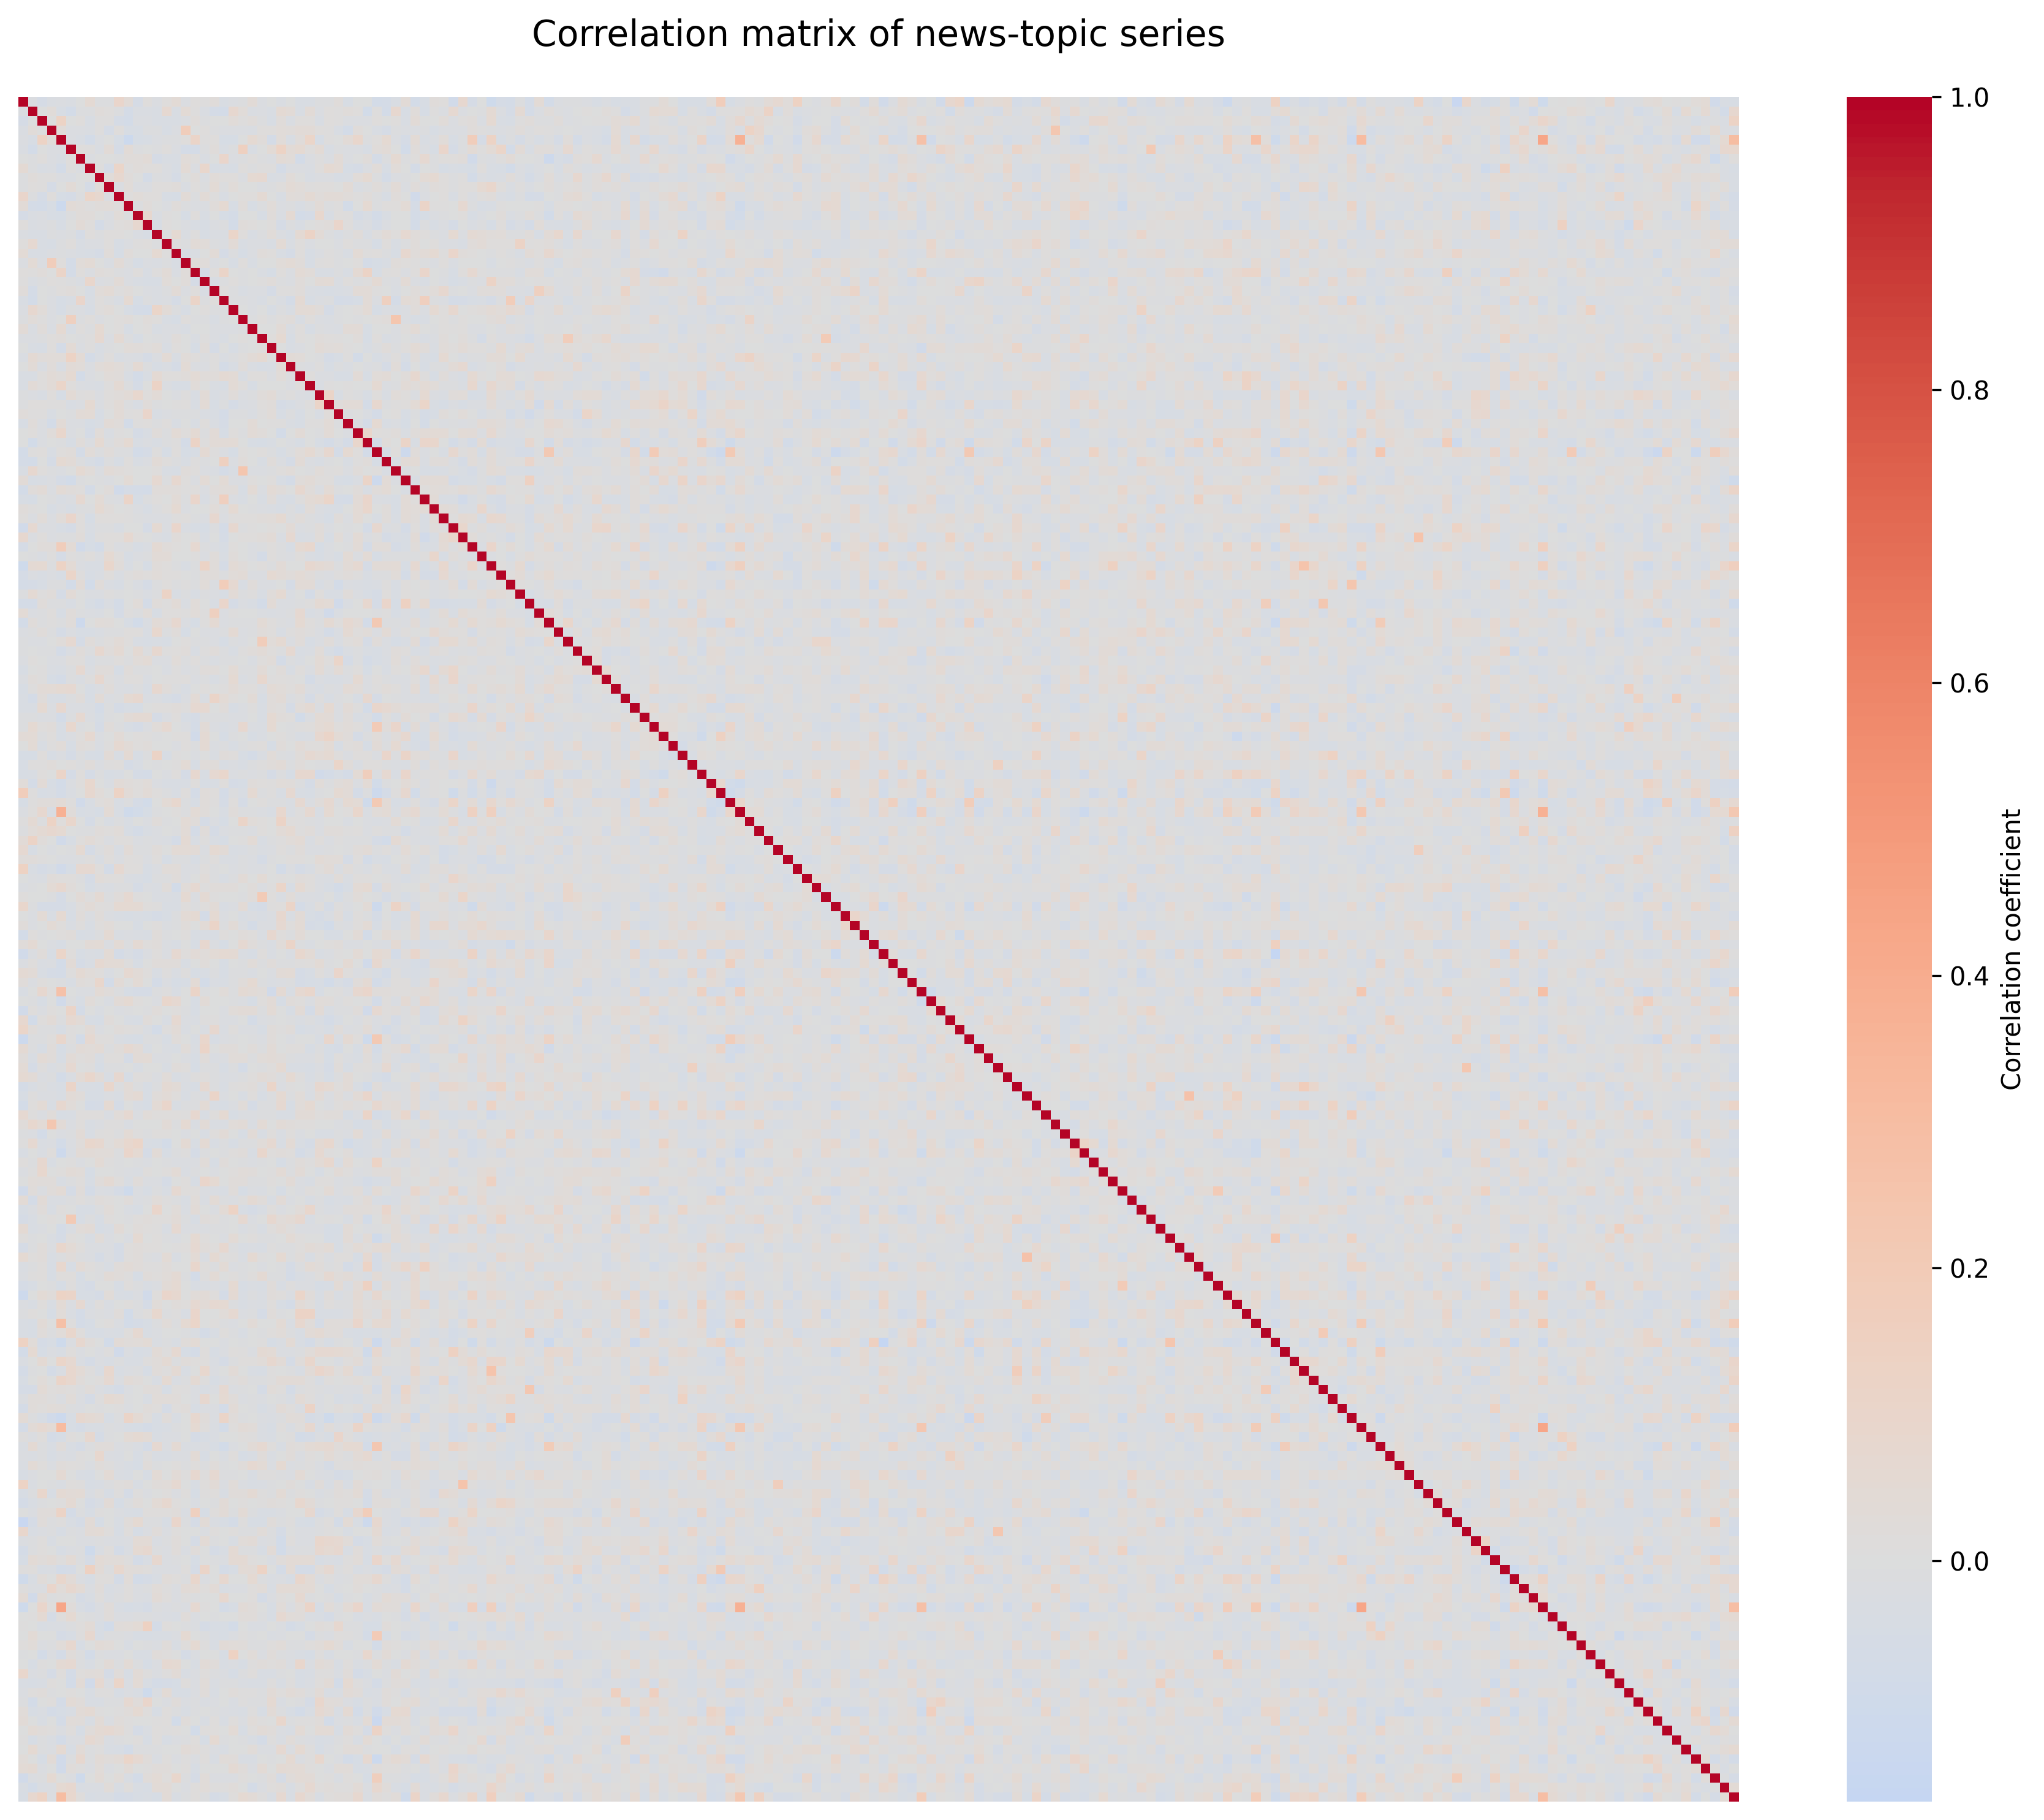
\includegraphics[width=\linewidth]{heatmap.png}
  \caption{Heatmap of correlation between news-topics.}
  \label{fig:corr_heatmap}
\end{figure}


